\chapter{Cuatro principios en matemáticas}

\section{Principio de las casillas (principio de la pichonera)}

\begin{ejercicio}
Demuestra que de tres números enteros, hay dos cuya suma es par.
\end{ejercicio}
\vspace{2cm}

El principio de las casillas establece que si hay $n+1$ elementos repartidos en $n$ casillas, entonces hay una casilla que tiene al menos dos elementos.

Una versión más general nos dice que si hay $nk+1$ elementos repartidos en $n$ clases distintas, entonces debe haber por lo menos una clase con al menos $k+1$ elementos.

\begin{ejercicio}
Muestra que en un conjunto de 25 personas hay tres que tienen el mismo signo zodiacal.
\end{ejercicio}
\vspace{2cm}

\begin{ejercicio}
A un auditorio asistieron 367 personas. Demuestra que hay dos que tienen el mismo cumpleaños
\end{ejercicio}
\vspace{2cm}

Nota: Comparar con el problema probabilístico. Bastan 23 personas para que la probabilidad de que dos de ellas tengan el mismo cumpleaños supere $\frac{1}{2}$.

\begin{ejercicio}
La ciudad de México tiene más de 16 millones de habitantes. Es conocido que una persona tiene menos de un millón de cabellos. Demuestra que hay al menos 17 personas con la misma cantidad de cabellos 
\end{ejercicio}
\vspace{2cm}

\begin{ejercicio}
Una bolsa contiene suficientes canicas negras y blancas. ¿Cuál es el mínimo número de pelotas que se tienen que extraer para garantizar que se hayan elegido al menos dos de un mismo color?

¿y para garantizar diez de un mismo color?

¿Y en la bolsa también hubieran suficientes canicas rojas?
\end{ejercicio}
\vspace{2cm}

El principio de las casillas también admite otras variaciones:

Si se reparten $n-1$ elementos en $n$ casillas, entonces necesariamente hay una casilla vacía.

O bien, más generalmente, si se reparten $kn-1$ elementos en $n$ casillas, entonces necesariamente hay una casilla con a lo más $k-1$ elementos.
\vspace{2cm}


El principio es bastante sencillo, lo que a veces es muy ingenioso es determinar cuales son las casillas que nos ayudan a resolver el problema.

\begin{ejercicio}
Se te otorga una lista de doce números enteros. Muestra que hay dos cuya diferencia es divisible entre $11$.
\end{ejercicio}
\vspace{2cm}

\begin{ejercicio}
Se te otorga una colección de $5$ puntos en el plano con coordenadas enteras. Muestra que algún punto medio de dos de esos puntos también tiene coordenadas enteras.
\end{ejercicio}
\vspace{2cm}

\begin{problema} [OMM '90]
Se tienen 19 puntos en el plano con coordenadas enteras. Muestra que se pueden elegir tres puntos cuyo centro de gravedad también tiene coordenadas enteras.
\end{problema}
\vspace{2cm}
\newpage

\begin{ejercicio}
¿Cuál es el máximo número de reyes que se pueden colocar en un tablero de ajedrez sin que estos se ataquen entre sí? 
\end{ejercicio}
%Sug: Se pueden poner $16$ con un acomodo regular. Casillas de $2\times 2$ muestra que no es posible con $17$.

  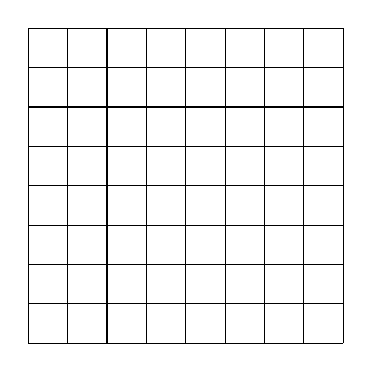
\begin{tikzpicture}[x=0.5cm,y=0.5cm]
     \foreach \i in {0,...,8} \draw[black] (0,\i) -- (8,\i);
    \foreach \i in {0,...,8} \draw[black] (\i,0) -- (\i,8);       
  \end{tikzpicture}
  
  

\begin{ejercicio}
¿Cuál es el máximo número de casillas que se pueden colorear en un tablero de ajedrez de tal manera que si se coloca cualquier triminó sobre el tablero, cubra al menos un cuadrito sin colorear?
\end{ejercicio}
%Sug: Se pueden colorear $32$ (ajedrez). Casillas de $2\times 2$ muestran que no es posible con $33$.

\begin{proposicion}
[Lema de los saludos I]
Demuestra que en una reunión de $n$ personas, en todo momento hay dos personas que han saludado a la misma cantidad de personas.
\end{proposicion}
\vspace{2cm}

\begin{ejercicio}
Los cuadritos de una cuadrícula de $3\times 7$ se colorean de rojo o azul. Muestra que hay un rectángulo con sus 4 esquinas del mismo color. 
\end{ejercicio}
  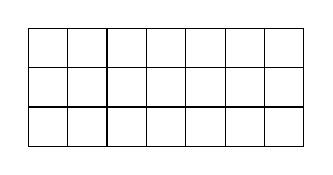
\begin{tikzpicture}[x=0.5cm,y=0.5cm]
     \foreach \i in {0,...,3} \draw[black] (0,\i) -- (7,\i);
    \foreach \i in {0,...,7} \draw[black] (\i,0) -- (\i,3);       
  \end{tikzpicture}

\begin{ejercicio}
Los cuadritos de una cuadrícula de $19\times 4$ se colorean de rojo, azul o verde. Muestra que hay un rectángulo con sus 4 esquinas del mismo color. 
\end{ejercicio}
%Sug: En cada columna domina un color. Combinaciones de 4 en 2 da seis.
  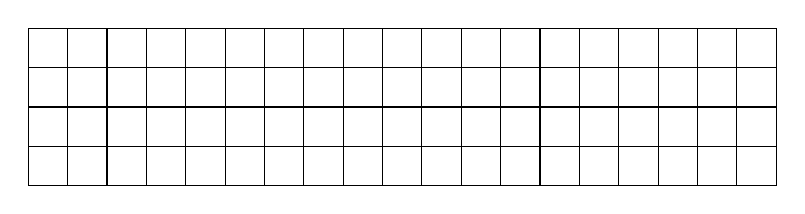
\begin{tikzpicture}[x=0.5cm,y=0.5cm]
     \foreach \i in {0,...,4} \draw[black] (0,\i) -- (19,\i);
    \foreach \i in {0,...,19} \draw[black] (\i,0) -- (\i,4);       
  \end{tikzpicture}

\begin{problema}
En una cuadrícula de $8\times 8$ se han escogido arbitrariamente diez cuadritos y se han marcado sus centros. Demuestra que, o bien existen dos puntos marcados con distancia menor o igual que $\sqrt{2}$, o bien algún punto marcado se encuentra a distancia $\frac{1}{2}$ del borde de la cuadrícula. 
\end{problema}
  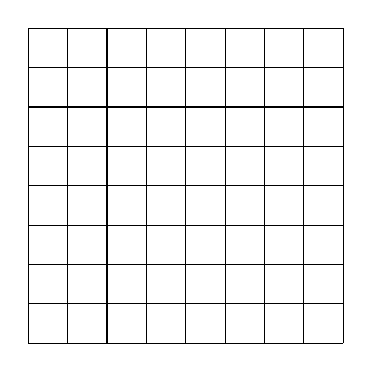
\begin{tikzpicture}[x=0.5cm,y=0.5cm]
     \foreach \i in {0,...,8} \draw[black] (0,\i) -- (8,\i);
    \foreach \i in {0,...,8} \draw[black] (\i,0) -- (\i,8);       
  \end{tikzpicture}
  
 
\begin{ejercicio}
Cinco puntos se colocan en un triángulo equilátero de lado $2$. Demuestra que hay dos puntos a distancia menor o igual $1$.
\end{ejercicio}
\vspace{2cm}

\begin{ejercicio}
Demuestra que un triángulo equilátero de lado $1$ no puede cubrirse completamente con dos triángulos equiláteros de lado menor.
\end{ejercicio}
\vspace{2cm}

\begin{ejercicio}
Se colocan siete puntos en un disco de radio $1$, de tal manera que la distancia entre cada par de ellos es mayor o igual a $1$. Demuestra que uno de los puntos tiene que ser el centro del círculo.
\end{ejercicio}
\vspace{2cm}

\begin{ejercicio}
Se colocan 501 tarjetas de tamaño $1\times 1$ sobre un recipiente en forma de prisma con base cuadrangular de $10\times 10$. Muestra que hay un punto de la base cuadrada que está cubierto por al menos 6 tarjetas.
\end{ejercicio}
\vspace{2cm}


\begin{ejercicio}
Se colocan 101 puntos en un cuadrado de lado $10$. Muestra que hay tres puntos que forman un triángulo de área menor o igual que 1.
\end{ejercicio}
\vspace{2cm}

\begin{ejercicio}
Se toman 8 números diferentes del conjunto $\{1, 2, 3, \dots , 14, 15 \}$. Demuestra que hay tres parejas usando esos números que tienen la misma diferencia (positiva) 
\end{ejercicio}
\vspace{2cm}

\newpage
\begin{problema}
Dado un conjunto de diez números de dos dígitos, mostrar que existen dos subconjuntos disjuntos con la misa suma.
\end{problema}
Sug: Las posibles sumas van de $0$ hasta $99+98+97+\cdots +90 < 1000$. ¿Cuántos subconjuntos hay?
\vspace{2cm}


\begin{ejercicio}
Hay 650 puntos dentro de un círculo de radio 16. Muestra que existe un anillo de radio interior 2 y radio exterior 3 que cubre al menos 10 puntos.
\end{ejercicio}
\vspace{2cm}

%Sug: Un anillo $R$ tapa a un punto $P$ si y solo si el anillo con centro en $P$ tapa al centro de $R$. 

\begin{problema}
Hay $33$ torres en un tablero de ajedrez. Muestra que hay un subconjunto de $5$ torres que no se atacan entre sí.
\end{problema}
%Sug: Si hay 9 torres hay dos distinta columna y dos en distinta fila. Si hay 17 torres, hay tres que no se atacan...


\newpage

Una {\bf gráfica} o {\bf grafo} (simple) es un conjunto de puntos $V=\{v_1, v_2,\dots, v_n \}$ llamados {\bf vértices} y un subconjunto de pares (no-ordenados) de vértices, llamados {\bf aristas}. 

A la gráfica de $n$-vértices que contiene a todas las aristas se le llama {\bf gráfica completa} o $K_n$.

\begin{tikzpicture}[line cap=round,line join=round,>=triangle 45,x=1.5cm,y=1.5cm]
\draw [line width=1.pt] (1.,0.)-- (-0.5,0.8660254037844387);
\draw [line width=1.pt] (-0.5,0.8660254037844387)-- (-0.5,-0.8660254037844385);
\draw [line width=1.pt] (-0.5,-0.8660254037844385)-- (1.,0.);
\draw [fill=black] (-0.5,0.8660254037844387) circle (1.5pt);
\draw [fill=black] (-0.5,-0.8660254037844385) circle (1.5pt);
\draw [fill=black] (1.,0.) circle (1.5pt);
\draw [fill=black] (1.,0.) circle (1.5pt);
\draw [fill=black] (-0.5,0.8660254037844387) circle (1.5pt);
\draw [fill=black] (-0.5,-0.8660254037844385) circle (1.5pt);
\end{tikzpicture}
\begin{tikzpicture}[line cap=round,line join=round,>=triangle 45,x=1.5cm,y=1.5cm]
\draw [line width=1.pt] (0.,-1.)-- (0.,1.);
\draw [line width=1.pt] (0.,1.)-- (-1.,0.);
\draw [line width=1.pt] (-1.,0.)-- (0.,-1.);
\draw [line width=1.pt] (0.,-1.)-- (1.,0.);
\draw [line width=1.pt] (1.,0.)-- (0.,1.);
\draw [line width=1.pt] (1.,0.)-- (-1.,0.);
\draw [fill=black] (0.,1.) circle (1.5pt);
\draw [fill=black] (-1.,0.) circle (1.5pt);
\draw [fill=black] (0.,-1.) circle (1.5pt);
\draw [fill=black] (0.,-1.) circle (1.5pt);
\draw [fill=black] (0.,1.) circle (1.5pt);
\draw [fill=black] (-1.,0.) circle (1.5pt);
\draw [fill=black] (1.,0.) circle (1.5pt);
\draw [fill=black] (1.,0.) circle (1.5pt);
\end{tikzpicture}
\begin{tikzpicture}[line cap=round,line join=round,>=triangle 45,x=1.5cm,y=1.5cm]
\draw [line width=1.pt] (-0.8090169943749475,-0.587785252292473)-- (0.30901699437494745,0.9510565162951535);
\draw [line width=1.pt] (0.30901699437494745,0.9510565162951535)-- (-0.8090169943749473,0.5877852522924732);
\draw [line width=1.pt] (-0.8090169943749473,0.5877852522924732)-- (-0.8090169943749475,-0.587785252292473);
\draw [line width=1.pt] (-0.8090169943749475,-0.587785252292473)-- (0.30901699437494723,-0.9510565162951536);
\draw [line width=1.pt] (0.30901699437494723,-0.9510565162951536)-- (0.30901699437494745,0.9510565162951535);
\draw [line width=1.pt] (0.30901699437494723,-0.9510565162951536)-- (-0.8090169943749473,0.5877852522924732);
\draw [line width=1.pt] (0.30901699437494745,0.9510565162951535)-- (1.,0.);
\draw [line width=1.pt] (1.,0.)-- (-0.8090169943749473,0.5877852522924732);
\draw [line width=1.pt] (1.,0.)-- (-0.8090169943749475,-0.587785252292473);
\draw [line width=1.pt] (1.,0.)-- (0.30901699437494723,-0.9510565162951536);
\draw [fill=black] (0.30901699437494745,0.9510565162951535) circle (1.5pt);
\draw [fill=black] (-0.8090169943749473,0.5877852522924732) circle (1.5pt);
\draw [fill=black] (-0.8090169943749475,-0.587785252292473) circle (1.5pt);
\draw [fill=black] (-0.8090169943749475,-0.587785252292473) circle (1.5pt);
\draw [fill=black] (0.30901699437494745,0.9510565162951535) circle (1.5pt);
\draw [fill=black] (-0.8090169943749473,0.5877852522924732) circle (1.5pt);
\draw [fill=black] (0.30901699437494723,-0.9510565162951536) circle (1.5pt);
\draw [fill=black] (0.30901699437494723,-0.9510565162951536) circle (1.5pt);
\draw [fill=black] (1.,0.) circle (1.5pt);
\draw [fill=black] (1.,0.) circle (1.5pt);
\end{tikzpicture}
\begin{tikzpicture}[line cap=round,line join=round,>=triangle 45,x=1.5cm,y=1.5cm]
\draw [line width=1.pt] (-1.,0.)-- (0.5,0.8660254037844386);
\draw [line width=1.pt] (0.5,0.8660254037844386)-- (-0.5,0.8660254037844387);
\draw [line width=1.pt] (-0.5,0.8660254037844387)-- (-1.,0.);
\draw [line width=1.pt] (-1.,0.)-- (-0.5,-0.8660254037844385);
\draw [line width=1.pt] (-0.5,-0.8660254037844385)-- (0.5,0.8660254037844386);
\draw [line width=1.pt] (-0.5,-0.8660254037844385)-- (-0.5,0.8660254037844387);
\draw [line width=1.pt] (0.5,0.8660254037844386)-- (1.,0.);
\draw [line width=1.pt] (1.,0.)-- (-0.5,0.8660254037844387);
\draw [line width=1.pt] (1.,0.)-- (-1.,0.);
\draw [line width=1.pt] (1.,0.)-- (-0.5,-0.8660254037844385);
\draw [line width=1.pt] (0.5,-0.866025403784439)-- (-1.,0.);
\draw [line width=1.pt] (0.5,-0.866025403784439)-- (-0.5,0.8660254037844387);
\draw [line width=1.pt] (0.5,-0.866025403784439)-- (0.5,0.8660254037844386);
\draw [line width=1.pt] (0.5,-0.866025403784439)-- (-0.5,-0.8660254037844385);
\draw [line width=1.pt] (0.5,-0.866025403784439)-- (1.,0.);
\draw [fill=black] (0.5,0.8660254037844386) circle (1.5pt);
\draw [fill=black] (-0.5,0.8660254037844387) circle (1.5pt);
\draw [fill=black] (-1.,0.) circle (1.5pt);
\draw [fill=black] (-1.,0.) circle (1.5pt);
\draw [fill=black] (0.5,0.8660254037844386) circle (1.5pt);
\draw [fill=black] (-0.5,0.8660254037844387) circle (1.5pt);
\draw [fill=black] (-0.5,-0.8660254037844385) circle (1.5pt);
\draw [fill=black] (-0.5,-0.8660254037844385) circle (1.5pt);
\draw [fill=black] (1.,0.) circle (1.5pt);
\draw [fill=black] (1.,0.) circle (1.5pt);
\draw [fill=black] (0.5,-0.866025403784439) circle (1.5pt);
\draw [fill=black] (0.5,-0.866025403784439) circle (1.5pt);
\end{tikzpicture}

\begin{ejercicio}
Colorea las aristas del $K_5$ de manera que no se forme un triángulo monocromático.
\end{ejercicio}

\begin{ejercicio}
Demuestra que si se colorean las aristas del $K_6$ de dos colores, entonces forzosamente se forma un triángulo monocromático.
\end{ejercicio}
\vspace{4cm}

Para $n,m\geq 1$, el {\bf número de Ramsey} $R(n,m)=R$ se define como el número natural más pequeño tal que, de colorearse las aristas de un $K_R$ con rojo y azul, entonces se garantiza la existencia de un $K_n$ rojo o bien de un $K_m$ azul.

Los dos ejercicios anteriores juntos significan justamente que el número de Ramsey $R(3,3)=6$.
\newpage

\begin{ejercicio}
Para todo $n,m\geq 1$, $R(n,1)= 1$ y $R(1,m)=1$.
\end{ejercicio}
\vspace{2cm}

\begin{ejercicio}
Sea $m\geq 2$. Demuestra que $R(2,m)= m$.
\end{ejercicio}
\vspace{2cm}

\begin{ejercicio}
Demuestra que si se colorean las aristas del $K_{10}$ de dos colores, entonces forzosamente se forma un $K_3$ rojo, o un $K_4$ azul.
\end{ejercicio}
\vspace{2cm}

Observa que el ejercicio anterior muestra que $R(3,4)\leq 10$. Más adelante mostraremos que $R(3,4)\leq 9$. Como es posible encontrar una coloración del $K_8$ sin un triángulo rojo ni un $K_4$ azul, se concluye que $R(3,4)=9$.

En general se pueden encontrar cotas sencillas para los números de Ramsey:

\begin{ejercicio}
Demuestra que $R(m,n)\leq R(m-1,n)+ R(m,n-1)$.
\end{ejercicio}
\vspace{2cm}

Se pueden considerar más colores:

\begin{ejercicio}
Demuestra que si se colorean las aristas del $K_{17}$ de tres colores, entonces forzosamente se forma un triángulo monocromático.
\end{ejercicio}
\vspace{2cm}

\begin{proposicion}
[Lema de los saludos II / Handshaking Lemma]
Demuestra que en una reunión de $n$ personas, en todo momento hay siempre una cantidad par de personas que han saludado a un número impar de personas.
\end{proposicion}
\vspace{2cm}

\begin{ejercicio}
Demuestra que si se colorean las aristas del $K_{9}$ de dos colores, entonces forzosamente se forma un triángulo rojo, o un $K_4$ azul.
\end{ejercicio}
\vspace{2cm}

De hecho, el resultado anterior es un caso particular del siguiente:

\begin{proposicion}
Si tanto $R(m-1,n)$ como $R(m,n-1)$ son pares, entonces se cumple que $R(m,n)\leq R(m-1,n)+R(m,n-1)-1$
\end{proposicion}
La demostración se deja como ejercicio.
\vspace{2cm}

Usando los resultados anteriores se puede deducir que $R(4,4)\leq R(4,3)+R(3,4)=18$.

De todas las $6.4\times 10^{22}$ posibles bi-coloraciones de las aristas del $K_{16}$, solamente hay dos que no contienen un $K_4$ monocromático. De todas las $2.46 \times 10^{26}$ posibles bi-coloraciones de aristas del $K_{17}$, solamente hay una que no tiene un $K_4$ monocromático, estableciendo así que $R(4,4)=18$ (1979). En 1995 se demostró que $R(4,5)=25$. De $R(5,5)$ solamente sabemos que $43\leq R(5,5)\leq 48$

Sobre la complejidad de calcular numeros de Ramsey:

\epigraph{Paul Erdös nos pide imaginarnos que una civilización extraterrestre, mucho más poderosa que la nuestra, ha aterrizado en nuestro planeta, demandándonos calcular $R(5,5)$ para mostrarles que somos vida inteligente y no destruirnos. En ese caso, nos sugiere poner a todos nuestros científicos y a todas nuestras computadoras a intentar calcular ese valor. Si en cambio, nos exigieran calcular $R(6,6)$, él considera mucho más viable intentar destruir a los invasores.}{Joel Spencer}

\begin{problema}
[OMM '98] Se colorean todas las aristas de un $K_8$ con dos colores. Mostrar que existen al menos siete triángulos monocromáticos.
\end{problema}
\vspace{2cm}

En lugar de colorear aristas, el teorema de Ramsey también permite colorear caras de dimensiones mayores. El caso que ya estudiamos $R^d(m,n)$ corresponde a $d=2$. Para dimensión $d=3$ los números de Ramsey se definen de la siguiente manera.

Una $3$-hipergráfica completa $K^3_n$ es un conjunto de $n$ vértices junto con todas sus 3-caras (subconjuntos de 3 vértices).

\begin{ejercicio}
Si $m\geq 3$, $R^{d=3}(m,3)=m=R^{d=3}(3,m)$
\end{ejercicio}
\vspace{2cm}

\begin{problema}
Muestra que $R^{d=3}(4,4)\leq R^{d=2}(4,4)+1$
\end{problema}
\vspace{2cm}

\begin{problema}
Muestra que $R^{d=4}(5,5)\leq R^{d=3}(5,5)+1$
\end{problema}
\vspace{2cm}

\begin{problema}
Demuestra que para todo número natural $k\geq 1$ existe un $N$ suficientemente grande tal que para cualquier configuración de $N$ puntos en el plano en posición general, hay un subconjunto de $k$ puntos que forman un polígono convexo.
\end{problema}
Sug: $N=R^{d=4}(k,5)$ ¿Puede haber un subconjunto de 5 puntos donde todos los sub-cuadriláteros no sean convexos?.
\vspace{2cm}

\newpage

\section{Principio de inclusión y exclusión}

\section{Principio de inducción matemática}

\begin{ejercicio} Fibonacci:
¿Identidad de Cassini?, 

¿Identidad de Catalan?, 

¿Identidad de d'Ocagne?
\end{ejercicio}

%Revisar si tienen solución elemental, si no mover a inducción.


\section{Principio de invarianza}

\subsection*{Problemas de tableros}

\begin{problema}
A un tablero de ajedréz de $8\times 8$ se le remueven dos esquinas opuestas. ¿Se pueden cubrir todas las casillas con $31$ dominós de $2\times 1$?
\end{problema}
%Sug: de qué color son las esquinas que se removieron?.

\begin{problema}
¿Se puede formar un rectángulo usando una sola vez, sin traslaparse, cada una de las seis fichas del tetris?

\begin{tikzpicture}[line cap=round,line join=round,>=triangle 45,x=.5cm,y=.5cm]
\draw [line width=1pt] (0,0)-- (2,0);
\draw [line width=1pt] (0,0)-- (0,2);
\draw [line width=1pt] (0,2)-- (2,2);
\draw [line width=1pt] (2,2)-- (2,0);
\draw [line width=1pt] (0,1)-- (2,1);
\draw [line width=1pt] (1,2)-- (1,0);
\draw [line width=1pt] (5.6,2.6)-- (7.6,2.6);
\draw [line width=1pt] (7.6,2.6)-- (7.6,0.6);
\draw [line width=1pt] (6.6,0.6)-- (8.6,0.6);
\draw [line width=1pt] (8.6,0.6)-- (8.6,1.6);
\draw [line width=1pt] (8.6,1.6)-- (5.6,1.6);
\draw [line width=1pt] (5.6,2.6)-- (5.6,1.6);
\draw [line width=1pt] (6.6,2.6)-- (6.6,0.6);
\draw [line width=1pt] (0,4)-- (0,7);
\draw [line width=1pt] (0,7)-- (1,7);
\draw [line width=1pt] (1,7)-- (1,4);
\draw [line width=1pt] (1,4)-- (0,4);
\draw [line width=1pt] (0,5)-- (1,5);
\draw [line width=1pt] (1,6)-- (0,6);
\draw [line width=1pt] (5.9,4.7)-- (5.9,6.7);
\draw [line width=1pt] (5.9,6.7)-- (6.9,6.7);
\draw [line width=1pt] (6.9,6.7)-- (6.9,4.7);
\draw [line width=1pt] (7.9,5.7)-- (7.9,4.7);
\draw [line width=1pt] (8.9,5.7)-- (8.9,4.7);
\draw [line width=1pt] (8.9,5.7)-- (5.9,5.7);
\draw [line width=1pt] (5.9,4.7)-- (8.9,4.7);
\draw [line width=1pt] (4.5,1.2)-- (4.5,4.2);
\draw [line width=1pt] (3.5,4.2)-- (3.5,1.2);
\draw [line width=1pt] (2.5,3.2)-- (4.5,3.2);
\draw [line width=1pt] (2.5,2.2)-- (4.5,2.2);
\draw [line width=1pt] (2.5,3.2)-- (2.5,2.2);
\draw [line width=1pt] (3.5,4.2)-- (4.5,4.2);
\draw [line width=1pt] (3.5,1.2)-- (4.5,1.2);
\draw [line width=1pt] (2,7)-- (2,5);
\draw [line width=1pt] (3,5)-- (3,7);
\draw [line width=1pt] (2,7)-- (5,7);
\draw [line width=1pt] (5,6)-- (2,6);
\draw [line width=1pt] (2,5)-- (3,5);
\draw [line width=1pt] (4,7)-- (4,6);
\draw [line width=1pt] (5,7)-- (5,6);
\draw [line width=1pt] (0,4)-- (0,3);
\draw [line width=1pt] (0,3)-- (1,3);
\draw [line width=1pt] (1,3)-- (1,4);
\draw [fill=black] (0,0) circle (1.5pt);
\draw [fill=black] (1,0) circle (1.5pt);
\draw [fill=black] (2,0) circle (1.5pt);
\draw [fill=black] (0,1) circle (1.5pt);
\draw [fill=black] (1,1) circle (1.5pt);
\draw [fill=black] (2,1) circle (1.5pt);
\draw [fill=black] (2,2) circle (1.5pt);
\draw [fill=black] (1,2) circle (1.5pt);
\draw [fill=black] (0,2) circle (1.5pt);
\draw [fill=black] (0,4) circle (1.5pt);
\draw [fill=black] (0,5) circle (1.5pt);
\draw [fill=black] (0,6) circle (1.5pt);
\draw [fill=black] (0,7) circle (1.5pt);
\draw [fill=black] (1,6) circle (1.5pt);
\draw [fill=black] (1,5) circle (1.5pt);
\draw [fill=black] (1,4) circle (1.5pt);
\draw [fill=black] (1,7) circle (1.5pt);
\draw [fill=black] (2,6) circle (1.5pt);
\draw [fill=black] (2,7) circle (1.5pt);
\draw [fill=black] (3,7) circle (1.5pt);
\draw [fill=black] (4,7) circle (1.5pt);
\draw [fill=black] (5,7) circle (1.5pt);
\draw [fill=black] (5,6) circle (1.5pt);
\draw [fill=black] (4,6) circle (1.5pt);
\draw [fill=black] (3,6) circle (1.5pt);
\draw [fill=black] (2,5) circle (1.5pt);
\draw [fill=black] (3,5) circle (1.5pt);
\draw [fill=black] (5.9,6.7) circle (1.5pt);
\draw [fill=black] (5.9,5.7) circle (1.5pt);
\draw [fill=black] (6.9,5.7) circle (1.5pt);
\draw [fill=black] (6.9,6.7) circle (1.5pt);
\draw [fill=black] (5.9,4.7) circle (1.5pt);
\draw [fill=black] (6.9,4.7) circle (1.5pt);
\draw [fill=black] (7.9,4.7) circle (1.5pt);
\draw [fill=black] (8.9,4.7) circle (1.5pt);
\draw [fill=black] (8.9,5.7) circle (1.5pt);
\draw [fill=black] (7.9,5.7) circle (1.5pt);
\draw [fill=black] (5.6,2.6) circle (1.5pt);
\draw [fill=black] (6.6,2.6) circle (1.5pt);
\draw [fill=black] (7.6,2.6) circle (1.5pt);
\draw [fill=black] (6.6,1.6) circle (1.5pt);
\draw [fill=black] (5.6,1.6) circle (1.5pt);
\draw [fill=black] (6.6,0.6) circle (1.5pt);
\draw [fill=black] (7.6,0.6) circle (1.5pt);
\draw [fill=black] (8.6,0.6) circle (1.5pt);
\draw [fill=black] (8.6,1.6) circle (1.5pt);
\draw [fill=black] (7.6,1.6) circle (1.5pt);
\draw [fill=black] (2.5,3.2) circle (1.5pt);
\draw [fill=black] (3.5,4.2) circle (1.5pt);
\draw [fill=black] (4.5,4.2) circle (1.5pt);
\draw [fill=black] (3.5,3.2) circle (1.5pt);
\draw [fill=black] (3.5,2.2) circle (1.5pt);
\draw [fill=black] (4.5,2.2) circle (1.5pt);
\draw [fill=black] (2.5,2.2) circle (1.5pt);
\draw [fill=black] (3.5,1.2) circle (1.5pt);
\draw [fill=black] (4.5,1.2) circle (1.5pt);
\draw [fill=black] (4.5,3.2) circle (1.5pt);
\draw [fill=black] (0,3) circle (1.5pt);
\draw [fill=black] (1,3) circle (1.5pt);
\end{tikzpicture}

\end{problema}

%Sug: Tablero de ajedréz

\begin{problema}
¿Se puede cubrir un tablero de $7\times 7$ al que se le removieron tres esquinas, con $24$ dominós?
\end{problema}

%Sug: Tablero de ajedréz


\begin{problema}
¿Se puede cubrir un tablero $8\times 8$ con 15 tetraminos T y un tetramino cuadrado?.
\end{problema}

%Sug: Tablero de ajedréz


\begin{problema}
¿Se puede cubrir un tablero de $10\times 10$ con $25$ fichas de $1\times 4$?
\end{problema}

%Sug: Tablero de ajedréz doble, con cuadros negros y blacos de 2\times 2

\begin{problema}
¿Para qué valores de $n$ se puede cubrir un tablero de $n\times n$ sin las cuatro esquinas con L-tetraminos que no se traslapen?.
\end{problema}

%Sug: Se pueden los n=4k+2 (Mostrar construcción inductiva). Para descartar n=4k usar coloración por columnas + paridad.

\begin{problema}
Demuestra que no se puede cubrir un tablero de $4\times 11$ con once L-tetraminos.
\end{problema}

%Sug: Idem. Columnas o filas (una de las dos es la que sirve).

\begin{problema}
%[IWYMIC]
Se tienen muchas fichas de seis cuadritos como en el de la figura.

¿Es posible rellenar un rectángulo con una cantidad impar de esas fichas?. Justifica tu respuesta.

\begin{tikzpicture}[line cap=round,line join=round,>=triangle 45,x=.7cm,y=.7cm]
\draw [line width=1pt] (0,0)-- (0,2);
\draw [line width=1pt] (0,2)-- (2,2);
\draw [line width=1pt] (2,2)-- (2,0);
\draw [line width=1pt] (1,2)-- (1,0);
\draw [line width=1pt] (0,1)-- (4,1);
\draw [line width=1pt] (0,0)-- (4,0);
\draw [line width=1pt] (4,1)-- (4,0);
\draw [line width=1pt] (3,1)-- (3,0);
\draw [fill=black] (0,0) circle (1.5pt);
\draw [fill=black] (1,0) circle (1.5pt);
\draw [fill=black] (2,0) circle (1.5pt);
\draw [fill=black] (0,1) circle (1.5pt);
\draw [fill=black] (1,1) circle (1.5pt);
\draw [fill=black] (2,1) circle (1.5pt);
\draw [fill=black] (2,2) circle (1.5pt);
\draw [fill=black] (1,2) circle (1.5pt);
\draw [fill=black] (0,2) circle (1.5pt);
\draw [fill=black] (3,1) circle (1.5pt);
\draw [fill=black] (3,0) circle (1.5pt);
\draw [fill=black] (4,1) circle (1.5pt);
\draw [fill=black] (4,0) circle (1.5pt);
\end{tikzpicture}

\end{problema}

%Sug: Sí se puede. Sug2: Ej. con 15 fichas el de 9\times 10. ¿Mínimo??

\begin{problema}
Se puede cubrir un tablero de $5\times 5$, exceptuando un cuadrito de $1\times 1$, con $6$ tetraminos L.
¿Cuáles son las posibles posiciones del cuadrito de $1\times 1$?
\end{problema}

\begin{problema}
Una tablero de $7\times 7$ se puede cubrir con 16 fichas de $3\times 1$ y una ficha de $1\times 1$
¿Cuáles son las posibles posiciones del cuadrito de $1\times 1$?
\end{problema}

\begin{problema}
Para qué valores de $n, m$ se puede cubrir un tablero de $m\times n$ con fichas de $1\times k$
\end{problema}

\begin{problema}
Se tiene un tableros de $9\times 9$ con un insecto en cada casilla, cada insecto vuela a alguna casilla vecina con la que comparte solo un vértice (algunos insectos se mueven a la misma casilla). ¿Cuál es el mínimo número de casillas desocupadas?
\end{problema}

\begin{problema}
[OMM]
1999 fichas, 2 jugadores.
\end{problema}

\begin{problema}
[IMO]
Ganchos.
\end{problema}

